\documentclass[../main.tex]{subfiles}

\begin{document}
%%%%%%%%%%%%%%%%%%%%%%%%%%%%%%%%%%%%%%%%%%%%
%                                          %
% Vektoren, Matrizen und Gleichungssysteme %
%                                          %
%%%%%%%%%%%%%%%%%%%%%%%%%%%%%%%%%%%%%%%%%%%%

\chapter{Vektoren, Matrizen und Gleichungssysteme}

\section{Skalare und Vektoren}
\textbf{Skalar:} ist eine reelle (oder komplexe) Zahl. \\
\textbf{Vektor:} hat einen (reellen) Betrag und eine Richtung. \\
Wir betrachten Vektoren in der Ebene $\vec{a} \in \mathbb{R}^2$

\subsection{Vektoraddition}
$\vec{a}+\vec{b} = 
\begin{bmatrix}a_1 \\a_2 \end{bmatrix} +  
\begin{bmatrix}b_1 \\b_2\end{bmatrix} = 
\begin{bmatrix}a_1 + b_1 \\a_2 +b_2 \end{bmatrix}$

\subsection{Vektor mit Skalar multiplizieren}
$\lambda\vec{a} = \lambda 
\begin{bmatrix}a_1 \\a_2 \end{bmatrix} = 
\begin{bmatrix}\lambda a_1 \\\lambda a_2 \end{bmatrix}$

\subsection{Rechenregeln für das Rechnen mit Vektoren}
Zusammen mit dem Nullvektor (Neutralelement der Vektoraddition), 0, gelten die folgenden Regeln für das Rehcnen mit Vektoren: 
\begin{itemize}
    \item $\vec{a}+\vec{b}=\vec{b}+\vec{a}$ Kommuntativgesetz 
    \item $\vec{a}+(\vec{b}+\vec{c})=(\vec{a}+\vec{b})+\vec{c}$ Assoziativgesetz 
    \item $\vec{a}+0=\vec{a}$ Existenz eines Neutralelements 0 
    \item $\vec{a}+(-\vec{a})=0$ Existens des Inversen 
    \item $\lambda(\vec{a}+\vec{b})=\lambda\vec{a}+\lambda\vec{b}$ 
    \item $(\lambda+\mu)\vec{a}=\lambda\vec{a}+\mu\vec{a}$ 
    \item $(\lambda\mu)\vec{a}=\lambda(\mu\vec{a})=\mu(\lambda\vec{a})$ 
    \item $1\vec{a}=\vec{a}$
\end{itemize}

\subsection{Skalarprodukt}
Das Skalarprodukt zweier Vektoren $\vec{a}$ und $\vec{b}$ ist definiert durch 
$\vec{a}\bullet\vec{b}=|\vec{a}|\cdot|\vec{b}|\cdot\cos\phi$. Dabei ist $\phi$ der Winkel 
zwischen den Vektoren a und b. Beachte den Unterschied zwischen den Symbolen "$\bullet$" 
(Skalarprodukt zweier Vektoren) und "$\cdot$" (normales Produkt zweier reellen Zahlen).
Hier stehen $|\vec{a}|$ und $|\vec{b}|$ für die Längen von a und b. \\ [7pt]
$\vec{a}\bullet\vec{b} =
\begin{bmatrix}a_1 \\a_2 \end{bmatrix} \bullet
\begin{bmatrix}b_1 \\b_2 \end{bmatrix} =
a_1b_1+a_2b_2$

\subsection{Betrag (Länge) eines Vektors}
Mit Hilfe des Skalarprodukts lässt sich der Betrag a des Vektors $\vec{a}$ wie folgt definieren: \\ [7pt]
$a\equiv|a|=\sqrt{\vec{a}\bullet\vec{a}}$ oder $|\vec{a}|^2=\vec{a}\bullet\vec{a}$ \\ [7pt]
Dann gilt im 2D-Fall (Satz von Pythagoras): $a\equiv|a|=\sqrt{\vec{a}\bullet\vec{a}}=\sqrt{a_1^2+a_2^2}$


\subsection{Einheitsvektor}
$\vec{e}=$ Einheitsvektor \\
$|\vec{e}|=1$

\subsection{Rechenregeln für das Skalarprodukt und Einheitsvektor}
Für beliebige reelle Zahlen $\lambda$ sowie beliebige Vektoren $\vec{a}$,$\vec{b}$ und $\vec{c}$ gilt: 
\begin{itemize}
    \item $\vec{a}\bullet\vec{b}=\vec{b}\bullet\vec{a}$ Kommuntativgesetz
    \item $\vec{a}\bullet(b+c)=\vec{a}\bullet\vec{b}+\vec{a}\bullet\vec{c}$ Distributivgesetz
    \item $\lambda(\vec{a}\bullet\vec{b})=(\lambda\vec{a})\bullet\vec{b}=\vec{a}(\lambda\vec{b})$
\end{itemize}

\subsection{Paarweise Senkrechte Vektoren}
Zwei Vektoren $\vec{a}$ und $\vec{b}$ stehen genau dann senkrecht aufeinander, sind 
also orthogonal, falls ihr Skalarprodukt verschwindet. \\ [7pt]
$\vec{a}\bullet\vec{b}=0 \iff \vec{a}\perp\vec{b}$ \\ [7pt]
Hier haben wir angenommen, dass der Nullvektor zu jedem Vektor senkrecht steht.

\section{Matrizen}
Eine $(m\times n)$-Matrix ist ein rechteckiges Schema von Zahlen. Es besteht aus $m$ Zeilen
und $n$ Spalten. Das Element $a_{i,j}\in\mathbb{R}$ steht in der $i$. Zeile und der $j$. Spalte. \\ [7pt]
Für eine quadratische Matrix gilt $m=n$ \\ [7pt]
Der erste Index $i$ von $a_{i,j}$ ist der Zeilenindex, der zweite $j$ der Spaltenindex. \\ [7pt]
Man schreibt kurz auch $\mathbf{A}=[a_{i,j}]$. \\ [7pt]

$\mathbf{A}= 
\begin{bmatrix}
    a_{1,1} \;\; a_{1,2} \;\; a_{1,j} \;\; a_{1,n} \\
    a_{2,1} \;\; a_{2,2} \;\; a_{2,j} \;\; a_{2,n} \\
    a_{i,1} \;\; a_{i,2} \;\; a_{i,j} \;\; a_{i,n} \\
    a_{m,1} \;\; a_{m,2} \;\; a_{m,j} \;\; a_{m,n} \\
\end{bmatrix}$

\subsection{Matrizen addieren}
Matrixaddition ist nur definiert, wenn beide Matrizen dieselbe Dimension haben! \\ [7pt]

$\mathbf{A} + \mathbf{B}= 
\begin{bmatrix}
    a_{1,1} \;\; a_{1,2}\\
    a_{2,1} \;\; a_{2,2} 
\end{bmatrix} +  
\begin{bmatrix}
    b_{1,1} \;\; b_{1,2}\\
    b_{2,1} \;\; b_{2,2} 
\end{bmatrix} =
\begin{bmatrix}
    (a_{1,1}+b_{1,1}) \;\; (a_{1,2}+b_{1,2})\\
    (a_{2,1}+b_{2,1}) \;\; (a_{2,2}+b_{2,2}) 
\end{bmatrix}
$

\subsection{Matrix mit einer Zahl multiplizieren}
Eine $(m\times n)$-Matrizen $\mathbf{A}=[a_{i,j}]$ wird mit einer Zahl $\alpha\in\mathbb{R}$
multipliziert, indem man jedes Matrixelement mit dieser Zahl multipliziert. \\ [7pt]

$\alpha\mathbf{A}=\alpha
\begin{bmatrix}
    a_{1,1} \;\; a_{1,2}\\
    a_{2,1} \;\; a_{2,2} 
\end{bmatrix} =
\begin{bmatrix}
    \alpha a_{1,1} \;\; \alpha a_{1,2}\\
    \alpha a_{2,1} \;\; \alpha a_{2,2} 
\end{bmatrix}$

\subsection{Rechnen mit Matrizen}
\begin{itemize}
    \item Durch die Matrixaddition wird zwei $(m\times n)$-Matrizen wieder eine $(m\times n)$-Matrix zugeordnet.
    \item Die \textbf{Nullmatrix} (d.h. eine Matrix mit lauter Nullen) ist das \textbf{Neutralelement} der Matrixaddition: $\mathbf{A+0}=\mathbf{0+A}=\mathbf{A}$.
    \item Das Negative einer Matrix \textbf{A} ist die Matrix, bei der jedes Matrixelement mit $(-1)$ multipliziert wird: $\mathbf{A}=(a_{i,j})\to -\mathbf{A}=(-a_{i,j})$. Man nennt $\mathbf{A}$ das \textbf{Inverse} von $\mathbf{A}$ bezüglich Addition.
    \item Die Subtraktion ist definiert durch $\mathbf{A-B}:=\mathbf{A}+(-1)\mathbf{B}$. Addiere zu $\mathbf{A}$ das Negative der Matrix $\mathbf{B}$
    \item \textbf{Assoziativgesetz}: $\mathbf{A}+(\mathbf{B}+\mathbf{C})=(\mathbf{A}+\mathbf{B})+\mathbf{C}$
    \item \textbf{Kommutativgesetz}: $\mathbf{A}+\mathbf{B} = \mathbf{B}+\mathbf{A}$
\end{itemize}

\subsection{Matrix mit Vektor multiplizieren}
Eine $(m\times n)$-Matrizen $\mathbf{A}=[a_{i,j}]$ wird mit einem $n$-dimensionalen (Spalten-) Vektor $\vec{x}$ wie folgt multipliziert: \\ [7pt]

$\mathbf{A} \vec{x}=
\begin{bmatrix}
    a_{1,1} \;\; a_{1,2}\\
    a_{2,1} \;\; a_{2,2} 
\end{bmatrix}
\begin{bmatrix}
    x_{1} \\
    x_{2}
\end{bmatrix} =
\begin{bmatrix}
    x_{1} a_{1,1} \;\; x_{2} a_{1,2}\\
    x_{1} a_{2,1} \;\; x_{2} a_{2,2} 
\end{bmatrix}$

\subsection{Matrixmultiplikation}
Das Produkt der (m$\times$n)-Matrix $A=[a_{i,j}]$ und der (n$\times$p)-Matrix $B=[ab_{i,j}]$ ist eine (m$\times$p)-Matrix $C=[c_{i,j}]$ definiert durch: \\
$C=AB=[c_{i,j}]$ wobei 
$c_{i,j}=a_{i,1}b_{1,j}+a_{i,2}b_{2,j}+...a_{i,k}b_{k,j}=$
$\sum\limits_{l=1}^ka_{i,l}b_{l,j}$ 
\begin{itemize}
    \item $c_{i,j}$ ist das Skalarprodukt des $i$ Zeilenvektors von $A$ mit dem $j$. Spaltenvektor von $B$.
    \item Beachte: Anzahl Spalten von $A$ (n) müssen mit der Anzahl Zeilen von $B$ (n) übereinstimmen um die beiden Matrizen multiplizieren zu können.
\end{itemize}
\subsubsection{Beispiel}
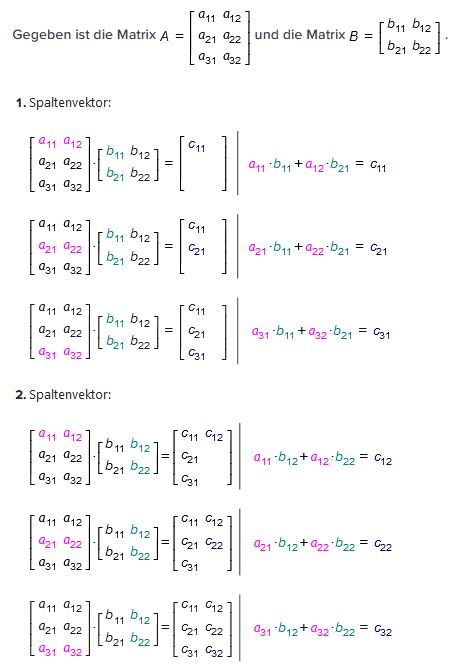
\includegraphics{matrizen_multiplikation.JPG}



\section{Gleichungssysteme}
\subsection{Lineare Gleichung}
Allgemeine Form: $ax+b=0$





\end{document}